\section{Detecting slower workers in operators}
    \subsection{First to finish application}
        Next, we provide a synthetic application modeling an application that can be modeled by a first to finish operator. \\
        Recall the previous FTF graph \cref{fig:ftf}. Assume a send request to ``the cloud'' that waits for a response or a timeout, it is modeled by an FTF operator. \cite{dq-tut}
       \subsubsection{Using the wrong operator}
            What happens if the wrong operator is chosen to represent the causal relationships between the outcomes? What if the user believes that the system diagram is the one we presented before in \cref{fig:mm1k} (1 in \cref{code:wrong_od})? The result on the oscilloscope will clearly show that something is wrong.
            \begin{figure}[H]
            \begin{minted}{text}
                ftf = worker_1 -> worker_2; (1)
                ... = f:ftf(worker_1, worker_2); (2)
            \end{minted}
            \caption{Two outcome diagram definitions proposed by the engineer for ftf.}
                \label{code:wrong_od}
            \end{figure}

            On the left in \cref{fig:ftf_osc}, we can observe how the sampling window \textbf{calculated $\Delta$Q} and its confidence bounds (2) are clearly greater than the sampling window \textbf{observed $\Delta$Q} (1) and its confidence bounds. This difference tells us that the proposed outcome diagram does not correctly represent the actual system. On the right, if no dependencies are present and the correct operator is chosen (2 in \cref{code:wrong_od}), the two $\Delta$Qs (observed and calculated) will overlap, as shown on the right in \cref{fig:ftf_osc}.

            \begin{figure}[H]
                \centering
                \begin{subfigure}{.5\textwidth}
                    \centering
                    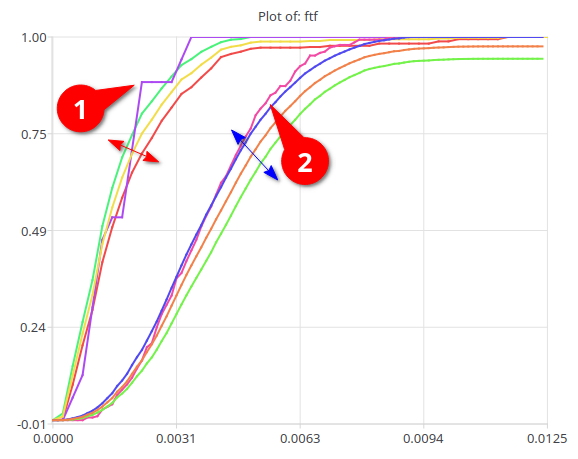
\includegraphics[width =0.98\textwidth]{img/bad1.png}
                    \label{fig:bad}
                \end{subfigure}%
                \begin{subfigure}{.5\textwidth}%
                    \centering%
                    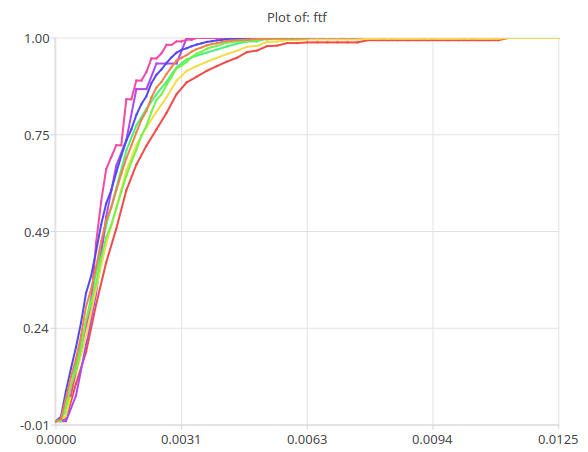
\includegraphics[width =0.98\textwidth]{img/good.png}%
                    \label{fig:good}%
                \end{subfigure}%
                \caption{\textbf{Left}: FTF plot \textbf{with wrong outcome diagram definition} as shown in the oscilloscope. (1) Observed $\Delta$Q. (2) Calculated $\Delta$Q. \\
                \textbf{Right}: FTF plot \textbf{with correct outcome diagram definition} as shown in the oscilloscope. Observed $\Delta$Q and calculated $\Delta$Q overlapping.}
                \label{fig:ftf_osc}%
            \end{figure}%
        \subsubsection{Introducing a slower component}
            Let us introduce a slower worker into the system, we introduce an artificial delay into worker\_2 (about 20ms). If the oscilloscope works correctly, the paradigm operations are sound and no dependencies are present in the system, we should not see any difference in the observed and calculated $\Delta$Qs of the FTF operator. Moreover, the FTF $\Delta$Q should be overlaid on top of the slower worker (\texttt{worker\_1}). In \cref{fig:ftf_w1w2}, this is the case, the FTF operator can be overlaid on top of worker\_1's graph. 

            \begin{figure}[H]
                \centering 
                \begin{subfigure}{.5\textwidth}
                    \centering
                    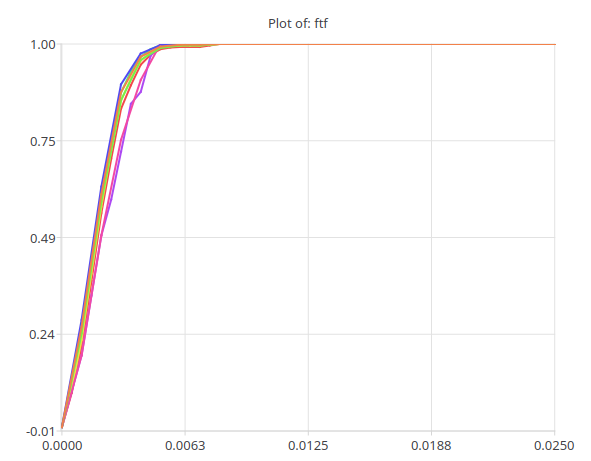
\includegraphics[width =0.98\textwidth]{img/ftf.png}
                    \label{fig:ftf_art_d}
                \end{subfigure}%
                \begin{subfigure}{.5\textwidth}%
                    \centering%
                    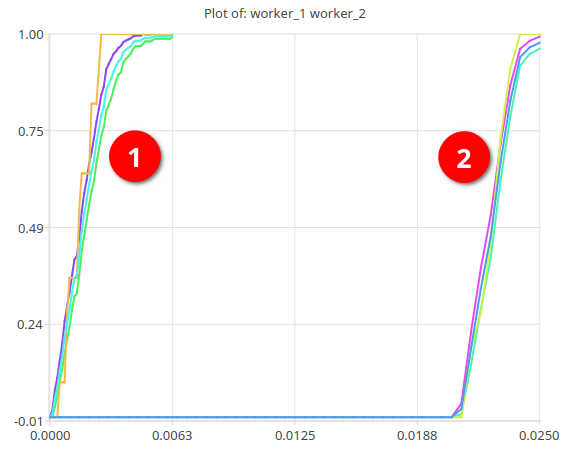
\includegraphics[width =0.98\textwidth]{img/delay32.png}%
                    \label{fig:ftf_art_dw}%
                \end{subfigure}%
                \caption{\textbf{Left}: FTF plot of worker\_1 and worker\_2, observed and calculated $\Delta$Q overlapping.\\
                \textbf{Right}: worker\_1 (1) and worker\_2 (2) $\Delta$Qs confidence bounds. \\
                The FTF plot correctly displays how worker\_2 does not have an effect on the FTF plot.}
                \label{fig:ftf_w1w2}%
            \end{figure}%

